\documentclass[11pt,a4paper]{article}

\usepackage[T1]{fontenc}
\usepackage[utf8]{inputenc}
\usepackage{mathptmx}
\usepackage{microtype}
\usepackage{amsmath,amssymb}
\usepackage{graphicx}
\usepackage[margin=2.7cm]{geometry}
\usepackage[colorlinks=true,allcolors=blue]{hyperref}
\hypersetup{pdftitle={When is anti-holomorphic dependence forced? The one-way
transfer kernel (v6)}, pdfauthor={Anthony Monnerot}}

\newcommand{\zb}{\bar{z}}
\newcommand{\wb}{\bar{w}}
\newcommand{\zbone}{\bar{z}_1}
\newcommand{\wbtwo}{\bar{w}_2}

\title{\bfseries When is anti-holomorphic dependence forced?\\
Exchange non-Hermiticity of one-way transfer kernels and a proposed
time-domain test in a recirculating fiber loop}
\author{Anthony Monnerot\\ \small Independent researcher, France}
\date{July 16, 2026 (v7)}

\begin{document}
\maketitle

\begin{abstract}
\noindent
We investigate when the anti-holomorphic (conjugate-variable) dependence of a
complex field or kernel is forced by the underlying physics, as opposed to being
removable by a choice of gauge, basis, or preparation. As a mathematical result, we
show that for two counter-winding mode ladders coupled unidirectionally --- via
reservoir-engineered, Lindblad-type coupling with a Jordan-block (double-pole)
structure per mode pair and a linear frequency ladder --- the two-point transfer
kernel sums to a closed form involving the Lerch transcendent in the product of
conjugated coordinates. Exchange-Hermiticity of the kernel and physical reciprocity are two
independent invariants: the reciprocity content is carried by the exchange
invariant $R = K - S(K)$ alone, evaluated on the complete two-point transfer
kernel, and exchange-Hermitian kernels exist that are not reciprocal (and
conversely), so the mirror partner certifies neither property by itself. The
one-way kernel violates both invariants: unidirectionality deletes the mirror
partner and, independently, makes $R \neq 0$. All symbolic claims are certified by exact Wirtinger-derivative
computation. We then propose an implementation in a recirculating fiber loop with
an intracavity amplifier and an in-loop isolator, together with a time-domain
protocol based on a secular revival envelope, a revival comb, and a
single-versus-twin-comb conditional reciprocity witness. Numerical simulations with
literature-typical component values indicate that the secular exponent remains
robust under several realistic noise sources, while revival-comb visibility is
significantly more demanding in terms of loop-phase stability. Beyond the protocol, we characterize the kernel's intrinsic analyticity boundary at $|x| = 1$ --- emergent from the mode ladder, with a chiral phase law of its branch-cut discontinuity separating the one-way kernel from its reciprocal control --- and prove an elementary Fourier floor theorem for the interference relief along the cut: the residual relief of large kernel sums is the window-contrast of the Fourier transform of the weighted winding measure, with closed-form floors for the canonical ladder families and a discreteness dichotomy (finite ladders keep their log-scale interference calendar forever; an absolutely continuous continuum forgets it). Read backwards, the law yields a spectroscopy of the surviving transfer element, recovering its winding measure from the relief alone, with proven limits. No experimental
measurements have been performed; experimental verification remains necessary.
\end{abstract}

\section{Introduction}

\subsection{The question}

A complex field or kernel on a two-dimensional carrier generally depends on both
the holomorphic coordinate $z$ and its conjugate $\zb$. In many physical settings
the anti-holomorphic dependence is an artifact of description: it can be removed
by a gauge transformation, by a change of basis, or by a different choice of
preparation or probe, after which the object is holomorphic, or real, or a
holomorphic function dressed by a modulus factor. This paper is concerned with
the opposite situation: when is the anti-holomorphic dependence \emph{forced} ---
present in every gauge, every basis, and for every admissible preparation? We treat
removability operationally: a structure is removable if some transformation
within a declared admissible class (unitary or similarity gauge
transformations, basis changes among the physical modes, choices of drive or
input port) maps the object to one whose mixed Wirtinger structure is trivial.
Forcedness is the failure of every such attempt, and we require it to be
certified symbolically rather than argued.

\subsection{Why one-point fields are insufficient}

Two elementary mechanisms empty the one-point case, and motivate the two-point
object studied here. First, reality locking: any physically real scalar
observable satisfies a conjugation constraint that ties its anti-holomorphic
content to its holomorphic content point by point; the two are mirror images
and carry no independent information. Second, preparation erasability: even for
a genuinely complex field obtained by driving a system, a one-point snapshot of
the driven response depends on the drive, and there exist admissible drives
that erase its anti-holomorphic content entirely; structure that can be
switched off by an input choice is not forced. Both mechanisms leave a natural
escape: an object that is neither a real observable nor a driven snapshot,
namely the two-point transfer kernel of an open, non-reciprocal system --- the
response at one point to a source at another. A kernel is a property of the
dynamical generator, not of any drive; and one-way coupling, implemented at
the level of the generator (Lindblad-type), deletes the conjugate-paired
sector that reality locking enforces and, independently, breaks the
reciprocity invariant $R = K - S(K)$ on the complete transfer kernel
(Section~\ref{sec:mirror}). The body of the
paper makes this escape quantitative.

\subsection{Results, and what is not claimed}

We establish, at the level of symbolically certified formula structure: (i) a
closed form for the two-point transfer kernel of two counter-winding mode
ladders under per-pair one-way Jordan coupling --- a Lerch transcendent in the
product of conjugated coordinates; (ii) an independence theorem --- exchange-Hermiticity
($\Delta = K - M(S(K))$) and reciprocity ($R = K - S(K)$) are independent
axes, all four zero/non-zero combinations being realized by certified
kernels, and
one-way coupling violates both, deleting the mirror partner and making
$R \neq 0$ on the complete transfer kernel; (iii) a three-fold classification of the
resulting kernel (conjugate-sector entanglement, non-pairing, transcendence)
with the paired-sum constructions as certified reciprocal counterexamples
and the reproducing-kernel (Bergman) form as the certified Hermitian decoy
($\Delta = 0$, $R \neq 0$). At the level of machine-verified simulation and one elementary hand proof, we further establish: (iv) the kernel's intrinsic, emergent analyticity boundary and the chiral phase law of its cut, with class-level genericity; (v) a Fourier floor theorem for the interference relief of large kernel sums, with sampling-dependent convergence rates and a discreteness dichotomy for the log-scale calendar; (vi) closed-form floors for the canonical ladder families; (vii) a spectroscopy of the surviving transfer element, with proven limits. We further propose a fiber-loop
implementation and a time-domain protocol, and we analyze its robustness
against literature-typical imperfections. We claim no experimental result: no
measurement has been performed, all component values are catalogue-typical, and
the relation of the kernel to superficially similar arithmetic objects (mock
modular forms) is discussed and explicitly not asserted. The contribution, if
any, is a sharply posed question, a certified structural dichotomy, an elementary machine-faced floor theorem with closed-form consequences, an inverse instrument whose limits are proven, and a
concrete, falsifiable measurement proposal.

Beyond the forcing question itself, the proposed protocol bears on an open
experimental debate in exceptional-point (EP) sensing. The claimed sensitivity
enhancement of EP-based sensors has been challenged on noise
grounds~\cite{Langbein2018,Wiersig2020}, and fundamental-limit analyses have
shown that non-reciprocity --- rather than EP proximity per se --- is the
resource that allows a sensor to exceed the bounds constraining any reciprocal
device~\cite{LauClerk2018}. Both strands of that debate presuppose the ability
to certify, in operation and under realistic noise, (i) that a device is
genuinely defective (a Jordan-block degeneracy rather than a near-degenerate
diagonalizable pair) and (ii) that it is genuinely non-reciprocal. The
time-domain observables proposed here address precisely these two
certification tasks at low cost: the secular exponent of the revival envelope
is a direct witness of Jordan structure which our simulations indicate is
robust to loop-phase jitter and between-shot noise (Section~\ref{sec:noise}),
and the single-versus-twin revival comb is, within the loop model, a
conditional witness of broken
reciprocity. We emphasize that these are certification tools; no
sensitivity-enhancement claim is made or implied.

\subsection{Outline}

Section~\ref{sec:structure} constructs the kernel and states the dichotomy.
Section~\ref{sec:boundary} characterizes the kernel's analyticity
boundary: its intrinsic and emergent character, the chiral phase law of
its cut, the interference relief along the tear, and the log-scale
calendar of its deep minima. Section~\ref{sec:floor} states and proves
the Fourier floor theorem, settles the fate of the calendar in the
continuum limit, and computes the canonical floors in closed form.
Section~\ref{sec:spectroscopy} reads the law backwards into a spectroscopy
of the surviving transfer element, with proven limits.
Section~\ref{sec:prior} situates the object among its nearest neighbors.
Section~\ref{sec:platform} describes the proposed platform and protocol;
Section~\ref{sec:noise} the imperfection analysis. Section~\ref{sec:discussion}
discusses assumptions, limitations, open questions, and falsifiability. The
certification details, the full proof of the floor theorem, the closed-form derivations, and the simulation
parameters are provided as supplementary material in the repository
accompanying this deposit.

\section{Mathematical structure of the one-way kernel}
\label{sec:structure}

\subsection{Setup}

We consider two families of modes with opposite winding on a ring-like carrier:
an ``upstream'' family $\phi_m \propto e^{+i m \theta}$ and a ``downstream''
family $\chi_m \propto e^{-i m \theta}$, indexed by $m \geq 1$. In complex
coordinates $z = r e^{i\theta}$ on (or near) the carrier circle, the upstream
family is holomorphic-like ($z^m$ up to a radial profile) and the downstream
family anti-holomorphic-like ($\zb^{\,m}$). Each pair $(\phi_m, \chi_m)$ is coupled
unidirectionally: the downstream mode is driven by the upstream one with
amplitude $g_m$, while the reverse matrix element vanishes identically. Such
one-way coupling can be produced by reservoir engineering in the sense of
cascaded quantum systems~\cite{Gardiner1993,Carmichael1993,MetelmannClerk2015}:
the vanishing of the reverse element is then a
property of the Lindblad generator itself, not of a drive or preparation
choice, which is the property we rely on throughout. When the two modes of a
pair are degenerate and damped at equal rates --- which is automatic if they are
frequency-degenerate partners coupled to the same bus --- the per-pair dynamical
matrix is triangular with equal diagonal entries, i.e., a $2\times 2$ Jordan block: the
transfer function from upstream to downstream carries a double pole,
\begin{equation}
G_m(\omega) \;=\; \frac{g_m}{\bigl(i(\omega - \omega_m) - \kappa/2\bigr)^{2}}.
\end{equation}
We take the pair frequencies on a linear ladder, $\omega_m = m\,\delta$ (free
spectral range $\delta$), with a common linewidth $\kappa$.

\subsection{Closed form of the two-point transfer kernel}
\label{sec:closedform}

The object of interest is not a one-point field but the two-point transfer
kernel: the response at observation point $\mathbf{r}_1$ to a localized source at
point $\mathbf{r}_2$. Writing the mode sums at fixed probe frequency and
collecting the winding bookkeeping (downstream factor $\zbone^{\,m}$ at the
observation point, conjugated upstream factor $\wbtwo^{\,m}$ at the source
point), the kernel takes the form
\begin{equation}
K(\mathbf{r}_1;\mathbf{r}_2) \;=\; \sum_{m \geq 1} g_m\, x^m,
\qquad x = \zbone\,\wbtwo,
\label{eq:kernelsum}
\end{equation}
convergent for $|x| < 1$ (observation and source inside the carrier circle).
We write $G_{21}$ for this surviving transfer element; the complete
two-channel kernel is the matrix $\mathbf{G} = (G_{ij})$ with $G_{12} = 0$,
and for matrix-valued kernels the exchange $S$ also transposes the channel
indices,
$(S \mathbf{G})_{ij}(\mathbf{r}_1, \mathbf{r}_2) = G_{ji}(\mathbf{r}_2,
\mathbf{r}_1)$, or explicitly in its $C$-covariant form
$(S_C \mathbf{G})(\mathbf{r}_1, \mathbf{r}_2) = C^{-1}\,
\mathbf{G}(\mathbf{r}_2, \mathbf{r}_1)^{T}\, C$: with this definition the
scalar element, a function of the commuting product $\zb\wb$, is
exchange-symmetric on its own, while the matrix kernel has
$R_{\mathbf{G}} = \mathbf{G} - S(\mathbf{G}) \neq 0$. In the general
statements of this paper $K$ denotes a generic two-point kernel --- scalar or
matrix, with $S$ acting accordingly --- and we write $G_{21}$ or $\mathbf{G}$
whenever the distinction matters; reciprocity statements always refer to the
matrix (Section~\ref{sec:mirror}). The
weight ladder determines the analytic class:
\begin{itemize}
\item[(a)] flat weights $g_m = g$ give the geometric (algebraic) kernel
  $g\,x/(1 - x)$;
\item[(b)] weights $g/m$ give the logarithmic kernel $-g \log(1 - x)$;
\item[(c)] the physical Jordan ladder $g_m = k / \lambda_m^2$ with
  $\lambda_m = -\kappa/2 - i m \delta$ gives
  \begin{equation}
  K \;=\; -\frac{k}{\delta^{2}} \left[\, \Phi(x, 2, c) - \frac{1}{c^{2}} \,\right],
  \qquad c = \frac{\kappa}{2 i \delta},
  \label{eq:lerch}
  \end{equation}
  where $\Phi$ is the Lerch transcendent; the leading structure is a
  dilogarithm.
\end{itemize}
Each closed form was verified against its defining series by partial-sum
comparison (forty terms, several sample points, geometric tail bound); we found
direct high-order numerical differentiation of the Lerch function unstable and
avoided it. We emphasize that case (a) shows the one-wayness of the kernel and
its transcendence are independent properties: flat weights produce a one-way
but algebraic kernel, and it is the physical double-pole ladder that supplies
the transcendental class.

\paragraph{Version note (v7).} This version repairs the reciprocity statement
of the published v3 (DOI 10.5281/zenodo.21317960). Exchange-Hermiticity and
reciprocity, stated as equivalent in v3 (abstract, contribution (ii), and this
section), are independent invariants; the Bergman reproducing kernel, used in
v3 as a reciprocal control, is exchange-Hermitian but not reciprocal
($\Delta = 0$, $R \neq 0$) and is reclassified below as the Hermitian decoy;
the reciprocity invariant must be evaluated on the complete two-point transfer
kernel, the scalar closed form being exchange-symmetric by itself; and the
cut-phase witness is stated comparatively, with its sufficiency-only limit
(Section~\ref{sec:chiral}). No closed form, simulation number, figure, or
protocol changed. The repair was prompted by an external adversarial audit and
is certified by an expanded repair harness built in the same exact symbolic
discipline as the original claims. Intermediate drafts v4--v6 existed only
internally and were never deposited.

\subsection{Reciprocity and exchange-Hermiticity: two independent invariants}
\label{sec:mirror}

Let $S$ denote the exchange of the two points, $(z, \zb) \leftrightarrow (w, \wb)$,
and let the mirror map $M$ act on a kernel formula by swapping each variable with
its conjugate together with $i \to -i$. We call a kernel
\emph{exchange-Hermitian} when $K = M(S(K))$ up to an additive constant; because
logarithmic branches can contribute a piecewise constant, the operationally safe
test is the constancy of $\exp\!\bigl(K - M(S(K))\bigr)$. Alongside
$\Delta = K - M(S(K))$ we define the \emph{reciprocity invariant}
$R = K - S(K)$: reciprocity is the statement $R = 0$ (the response from 2 to 1
equals the response from 1 to 2), while $\Delta = 0$ is an anti-linear
Hermiticity condition. These two invariants are \emph{independent} ---
conflating them was the error of earlier versions of this paper --- and all
four zero/non-zero combinations are realized by certified kernels:

\begin{center}
\begin{tabular}{lll}
\hline
quadrant & certified representative & invariants \\
\hline
reciprocal--Hermitian & $g(z,\zb) + g(w,\wb)$, real coefficient & $R = 0$, $\Delta = 0$ \\
dissipative reciprocal & $c\,(g(z,\zb) + g(w,\wb))$, $c \notin \mathbb{R}$, $M(g) = g$ & $R = 0$, $\Delta \neq 0$ \\
Hermitian decoy & Bergman $-k\log(1 - z\wb)$ & $R \neq 0$, $\Delta = 0$ \\
one-way & matrix kernel, $G_{21} = f(\zb\wb)$, $G_{12} = 0$ & $R \neq 0$, $\Delta \neq 0$ \\
\hline
\end{tabular}
\end{center}

The dissipative-reciprocal row requires the stated hypothesis: the complex
coefficient breaks $\Delta$ only if the building block is itself mirror-fixed
($M(g) = g$, $g \neq 0$); dissipation is fully compatible with reciprocity, a
point long emphasized in the electromagnetic literature
\cite{Caloz2018,Silveirinha2019}. At the operator level, with a symmetric
non-degenerate pairing $C$ and the reciprocal transpose
$A^{\sharp} = C^{-1} A^{T} C$ (no complex conjugation, hence loss-compatible),
$L = L^{\sharp}$ for the generator is equivalent to
$\mathbf{G} = \mathbf{G}^{\sharp}$ for the matrix kernel
$\mathbf{G} = L^{-1}$, i.e.\ to $R_{\mathbf{G}} = 0$; the identity
$(L^{-1})^{\sharp} = (L^{\sharp})^{-1}$ and the covariance $R' = U R U^{-1}$
under simultaneous transformation of $L$, $K$, $C$ are certified by the same
exact symbolic harness as the rest of the paper.

Two structural corollaries are certified with them, and the first is critical
for reading this paper. \emph{The object matters:} the one-way closed form is
a function of the single product $x = \zb\wb$, and the product commutes, so
the scalar closed form is exchange-\emph{symmetric} --- $R$ evaluated on it is
identically zero, a false ``reciprocal'' verdict. Non-reciprocity lives on the
complete two-point transfer kernel, the matrix with the reverse element
vanishing ($G_{21} = f(\zb\wb)$, $G_{12} = 0$), and only there is
$R \neq 0$. This realizes a general projection blindness: in the port basis
($C = I$) the diagonal of $R$ vanishes identically, and for a general
symmetric pairing the certified statement is $v^{T} C\,(K - K^{\sharp})\,v
= 0$ for every probe $v$ --- no same-port (one-point) measurement can ever
witness non-reciprocity; the invariant is irreducibly two-point. \emph{Second,} under
an external bias $b$ the Onsager--Casimir relation $K_b = K_{-b}^{\sharp}$
(device against bias-reversed device) must not be conflated with reciprocity
of the device against itself ($K_b = K_b^{\sharp}$): a gyrotropic kernel
satisfies the former while violating the latter.

We record the following observations, verified symbolically on all cases above
and on control kernels, organized by the two invariants. The diagonal
(reproducing-kernel) sum of a single holomorphic sector, $-k \log(1 - z\wb)$,
is exchange-Hermitian exactly --- yet, as a two-point kernel, non-reciprocal
($R \neq 0$): it realizes the Hermitian-decoy quadrant, and earlier versions
of this paper mislabeled it reciprocal; the Hermitian two-sector sum
(a one-way half plus its mirror image) is exchange-Hermitian with the paired
structure explicit; and the kernel $\log(z - \wb)$, which resembles
two-dimensional chiral propagators, is exchange-Hermitian up to a branch
constant ($\exp(\Delta) = -1$) and therefore lies on the Hermiticity axis up
to that constant; its $R$ is a separate question, not needed here.
Unidirectional coupling, by contrast, deletes the mirror partner: the one-way
kernels of Section~\ref{sec:closedform} satisfy no exchange-Hermiticity
relation, exactly because the reverse transfer element vanishes and nothing
restores the conjugate-exchanged term. We summarize this as: the mirror
partner marks exchange-Hermiticity, not reciprocity; the reciprocity statement
is carried by $R = K - S(K)$ on the complete transfer kernel. One-wayness
removes the partner and, independently, breaks $R$; the unpaired
anti-holomorphic half survives alone.

\subsection{Classification of the kernel}

The classification below concerns the scalar closed form (the content of the
surviving element $G_{21}$); the reciprocity statement lives on the matrix
kernel (Section~\ref{sec:mirror}). Three independent formula-level
properties position the one-way kernel. First,
cross-entanglement: the mixed logarithmic derivatives
$\partial_a \partial_b \log K$ across the two points, evaluated on all four
conjugate pairings $(z,w)$, $(z,\wb)$, $(\zb,w)$, $(\zb,\wb)$, vanish except on
$(\zb, \wb)$ --- the kernel is entangled between the two points, and
specifically in the doubly-conjugated sector, as the winding bookkeeping
dictates. (A single-pairing test is insufficient; we test all four.) Second,
non-pairing: $K$ is not invariant under the mirror map, and no mirror partner
accompanies it, in contrast with the exchange-Hermitian controls above. Third,
transcendence: for the physical ladder the closed form is a Lerch transcendent,
while the flat-weight control is algebraic; transcendence is an independent
axis supplied by the double-pole ladder. We do not attach any interpretation to
this classification beyond the statements just made.

\subsection{Certification methodology}

All symbolic statements above --- vanishing or non-vanishing of Wirtinger
derivatives, the pairing tests, the exchange-Hermiticity axis and the
independent reciprocity invariant $R$, including the branch-safe form --- are certified by exact symbolic computation of
Wirtinger derivatives (treating $z$, $\zb$, $w$, $\wb$ as independent
variables), in a fixed verification harness that also runs the control battery
(reproducing-kernel decoy, Hermitian paired sum, branch-constant case).
Numerical evidence (series verification, finite-difference cross-derivatives on
transcendental closed forms) supports but never replaces the symbolic
certificates. We adopt this separation --- a discoverer may propose, only the
symbolic judge certifies --- throughout the paper.

\section{Boundary structure of the kernel}
\label{sec:boundary}

The closed form of Section~\ref{sec:closedform} converges on the open unit
polydisk $|x| < 1$, $x = \zbone\wbtwo$, and the proposed protocol reads its
boundary values. This section records the machine-verified structure of that
boundary: its intrinsic and emergent character
(Section~\ref{sec:wall}), the chiral law of its crossing
(Section~\ref{sec:chiral}), the interference relief along its tear
(Section~\ref{sec:relief}), and the exact log-scale calendar of the deep
interference minima (Section~\ref{sec:calendar}). All results are
structural characterizations of the kernel, verified in the repository
accompanying this deposit; no physical claim is made.

\subsection{An intrinsic, emergent boundary}
\label{sec:wall}

Three structural facts about the boundary are worth
recording. First, the boundary is intrinsic and dimensionless: it sits at the
pure number $|x| = 1$, fixed by the geometry of the mode sum rather than by
any parameter choice (the physical rates $\kappa$ and $\delta$ enter the
complex offset $c$, not the location of the boundary), and the formalism
contains no dimensional constant from which any other distinguished scale
could be built. Second, the boundary is emergent in the mode ladder: every
truncation of the sum to $N$ rungs is an entire function of $x$ with no
boundary at all, while the radius at which the truncated sum departs from
the closed form approaches $|x| = 1$ monotonically as $N$ grows (at the
one-percent level, the departure radius is $0.904$ at $N = 10$ and $0.991$
at $N = 30$, and lies within $10^{-6}$ of the boundary beyond
$N \simeq 100$). The boundary is therefore a property of the infinite
ladder that no finite sub-ladder carries --- the domain-level analogue of
the fact, used throughout this section, that the one-way structure lives in
the full ladder rather than in any single Jordan pair. Third, the closed
form continues analytically beyond the boundary, where the defining series
diverges: the kernel as a function outlives the kernel as a mode sum, at
the price of a branch structure on $x \in (1, \infty)$ whose leading
discontinuity is inherited from the dilogarithm ($2\pi i \ln x$; we
verified the dilogarithm discontinuity numerically to nine digits, and
state the kernel-specific jump at the level of the Lerch-to-dilogarithm
reduction rather than as an independently certified result). We record
these facts as a structural characterization only: they sharpen, but do
not close, the boundary-limit question of Section~\ref{sec:discussion},
since a rigorous treatment of the $|x| \to 1$ limit in the presence of the
complex offset remains open.

These characterizations were subsequently audited at the class level.
The location of the boundary is dimensionless across coupling strengths
(departure radius $0.990636$ versus $0.987198$ at $N = 30$ for
$\kappa = 0.2$ and $\kappa = 1.0$), and, across ladder families, the
\emph{existence} of the wall is generic while its \emph{location} is set
by the asymptotics of the mode weights: polynomially decaying weights
place it at $|x| = 1$ for every tested power ($s = 1, 2, 3$, polylogarithm
controls), while geometrically decaying weights of ratio $r$ move it to
$|x| = 1/r$ (machine-checked at $r = 0.5$). The wall is a property of the
class; the choices pick the specimen.

\subsection{The chiral phase law of the cut}
\label{sec:chiral}

The crossing of the boundary is
\emph{oriented}: writing the leading discontinuity of the closed form
across the cut $x \in (1,\infty)$ as
$\mathrm{disc}\,\Phi(x,2,a) = 2\pi i\, x^{-a} \ln x$, the complex offset
$a = 1 + \kappa/(2i\delta)$ produced by one-way coupling makes the
\emph{phase} of the jump rotate along the cut (by
$\arg x^{-(a-1)}$, about $9.2^\circ$ from $x=1$ to $x=5$ at
$\kappa/\delta = 0.2$), whereas the real-offset dilogarithm control has a
frozen jump phase at every point of the cut. The ratio law
$\mathrm{disc}_{\text{one-way}}/\mathrm{disc}_{\text{reciprocal}}
= x^{-(a-1)}$ was verified digit-for-digit against the dilogarithm
control (itself machine-exact to $10^{-9}$); the monodromy stacking
across repeated crossings is arithmetic (equal sheet steps, ratios equal
to unity to $10^{-21}$). We are not aware of a published use of the
cut-discontinuity phase law, read comparatively across the two sectors, as a
(sufficient) reciprocity witness; the closest works
we found diagnose directionality through spectral winding numbers or
end-to-end Green's-function growth \cite{HuWang2023}, through the phase
of the drive \cite{McDonald2018}, or through a frequency-dependent
$2\pi$ phase gradient at a branch-cut crossing in non-Hermitian
metasurfaces \cite{Colom2023}; none states a position-dependent jump
phase along the cut, and we flag the usual caveat that niche
terminology may hide precedents.

Within the family studied here the reciprocal control has a real offset, so
the frozen-versus-rotating dichotomy separates the two kernels. The rotation
alone, however, is not a standalone reciprocity witness: for a separable
kernel $F_a(X) + F_a(Y)$ with the same complex offset in both sectors, each
sector carries the same rotating jump phase while the kernel is exactly
reciprocal ($R = 0$). The repaired witness is \emph{comparative}: with
$W(x) = D_X(x) - D_Y(x)$ the complex difference of the two sector jumps,
$W \neq 0$ implies $R \neq 0$ (the witness is sufficient), while $W = 0$ is
inconclusive --- an entire antisymmetric addition to the kernel changes $R$
without touching any cut (explicitly: $K_{\varepsilon} = \varepsilon\,(X -
Y)$ is entire, has zero cut discontinuity, and carries
$R = 2\varepsilon (X - Y) \neq 0$). The two sector cuts are compared with
the same orientation, fixed once by the common parametrization of $x$;
physically, the two sector jumps correspond to the two calibrated transfer
configurations ($G_{21}$ and $G_{12}$). The complex difference is essential: a size
asymmetry ($F_a(X) + \rho F_a(Y)$, $\rho > 0$ real, $\rho \neq 1$; a
unimodular complex $\rho$ would instead shift the weight angle, not the
size) leaves phase and slope identical in both sectors and is read only by
the modulus of $W$, with the
exact law $\max|W| = |1-\rho|\,|D|$. All clauses (refusal on the reciprocal
counterexample, firing on the one-way, size and speed columns, and the
inconclusive limit) are certified by the same exact symbolic harness. The
witness is established in the separable class $K = F(X) + G(Y)$ with two
sectors; outside that class the sector jumps need not be separately defined,
and no claim is made there.

The law was subsequently stress-tested across coupling strengths and
ladder families. The ratio identity holds to machine precision
($1.1\times10^{-16}$--$2.2\times10^{-16}$) at $\kappa = 0.05$, $0.2$ and
$1.0$, with the phase drift linear in the coupling,
$\arg x^{-(a-1)} = (\kappa/2\delta)\ln x$
($+0.99^\circ$, $+3.97^\circ$, $+19.86^\circ$ at $x = 2$ respectively);
and the drift law is independent of the weight family (polynomially
weighted ladders of every tested order obey the same law, with
polylogarithm controls agreeing to better than $10^{-9}$; the symbolic
identities are exact, the $10^{-9}$ figure is the numerical cross-check).
Within the family studied the twist separates the one-way kernel from its
real-offset control; it is not exclusive to the one-way class (a paired
reciprocal kernel with complex offset carries the same twist in both
sectors, Section~\ref{sec:chiral}), and only the comparative difference
witnesses $R$. The envelope belongs to the specimen.

\subsection{Interference relief along the cut}
\label{sec:relief}

When several kernels with
different ladder spacings are summed, their tears stack on the same ray
and the jumps add linearly, but the phase windings differ, and the
resulting interference relief along the cut is governed by a
\emph{detuning} law: at fixed spread of ladder spacings, increasing the
number of summed kernels averages the phases and flattens the relief,
whereas at fixed number, widening the spread of spacings builds it
(contrast growing by an order of magnitude and interior interference
extrema appearing), while the reciprocal control remains flat at
machine precision throughout. Together with the truncation behaviour of
Section~\ref{sec:wall}, this separates two emergence mechanisms living
on the same object: the boundary itself emerges from the \emph{number}
of rungs, while structure \emph{along} its tear emerges from their
\emph{diversity}. The emergence-with-$N$ pattern of an analyticity
boundary has well-known precedents in statistical mechanics --- the
accumulation of partition-function zeros in the thermodynamic limit
\cite{LeeYang1952} and the natural boundary of the 2D Ising
susceptibility built from singularities that become dense as the order
grows \cite{Nickel1999} --- and we present the truncation ladder of
Section~\ref{sec:wall} as an instance of that phenomenon in a
two-point transfer kernel with complex offset, not as a new class.

The relief was further dissected with respect to the weights of the
summed kernels. Positive real rescalings of the weights act as a volume
knob: interference minima keep their positions while only the contrast moves
(a negative real weight carries an angle $\pi$ and is not a pure volume
change). Relative complex phases between the weights reweight which minima
dominate rather than translating them --- a phase common to all weights
leaves the modulus relief invariant (the detailed window-dependence of the
relative-phase effect was diagnosed and is recorded in the repository). Size disparity alone
writes nothing: disparate weights on a single common winding speed give
contrast at machine zero ($9.6\times10^{-16}$), algebraically forced ---
the sum is a single fixed-length needle --- so winding-speed disparity
is the only source of relief. When sizes correlate with speeds the
response is asymmetric: weighting the slow windings collapses the
residual relief by an order of magnitude (a static-ballast effect:
quasi-static needles drown the relative ripples), while weighting the
fast ones raises it. Finally, as the number of summed kernels grows at
fixed spread, the relief does not vanish: it saturates toward a
distribution-dependent floor (near $0.048$ for log-uniformly spaced
ladders). The mechanism and the exact value of this floor admit a
closed law and an elementary theorem, developed in
Section~\ref{sec:floor}.

\subsection{The log-scale calendar of the deep rendezvous}
\label{sec:calendar}

The interference minima along the cut obey an exact and elementary law.
With the trivial $1/x$ envelope removed, the normalized relief of a sum
of $N$ kernels equals, for all $x > 1$,
\begin{equation}
P(u) \;=\; \Bigl|\,\sum_{k=1}^{N} w_k\, e^{\,i\nu_k u}\Bigr|,
\qquad u = \ln x,\qquad \nu_k = \frac{\kappa}{2\delta_k},
\label{eq:phasors}
\end{equation}
an algebraic identity rather than an asymptotic statement: the relief is
a finite sum of phasors rotating in \emph{logarithmic} scale,
almost-periodic in $u$ by construction. The deep minima are therefore
\emph{log-periodic} rendezvous of the phasors --- a form which is the
classical signature of complex exponents in the literature on discrete
scale invariance \cite{Derrida1984,Sornette1998}. Machine panels: for
$N = 2$ the relief is exactly periodic in $u$ with period
$T = 2\pi/|\nu_1 - \nu_2| = 94.247780$, matched to grid resolution; for
the three-ladder configuration used above, four deep minima occur at
$u = 10.00$, $29.98$, $49.93$, $69.81$ (spacings $\approx 19.9$, near
the extreme-winding beat), and the period law $T = 2\pi/|\Delta\nu|$
holds across four ladder spacings to $1.3\times10^{-3}$. This law also
resolves an earlier provisional reading: interference structures
reported at small $x$ in intermediate work were partial descents toward
the \emph{first} rendezvous (located near $x \approx 2.2\times10^{4}$ in
that configuration), outside every previously examined window; we record
the correction rather than the provisional reading. The calendar is
class-level --- independent of the weight family (an algebraic identity
in the $\nu_k$) and stable under fully randomized choirs of ladders ---
and it separates the kernel from its flat control: the real-offset control
(all $\nu_k = 0$) is flat to machine zero, with no minima at all.
Reciprocity by itself does not force $\nu_k = 0$ --- a paired reciprocal
kernel with rotating sectors carries a calendar too --- so the calendar,
like the twist, assigns one-wayness only through the comparative reading.

At the level of form, log-periodic oscillations are the hallmark of
discrete scale invariance, where complex exponents arise from
hierarchical structures or renormalization flows
\cite{Sornette1998,Derrida1984}. Here the imaginary part of the exponent
arises with no hierarchy anywhere in the construction --- in this model it
is produced by the one-way (Jordan) coupling, though complex winding is not
exclusive to one-way kernels (a paired reciprocal kernel with complex offset
carries it too, Section~\ref{sec:chiral}); to our knowledge this
hierarchy-free route to the motif is apparently new, and we flag the usual
caveat that niche terminology may hide precedents.



\section{The Fourier floor theorem}
\label{sec:floor}

Section~\ref{sec:relief} ended on an empirical fact: as the number of
summed kernels grows at fixed spread, the interference relief along the
cut saturates toward a distribution-dependent floor. This section derives
the exact law of that floor, proves it as an elementary theorem (the full
proof is deposited in the repository accompanying this record), settles
the fate of the log-scale calendar of Section~\ref{sec:calendar} in the
continuum limit, and computes the floors of the canonical ladder families
in closed form. Throughout, results labelled machine-verified were run
against the harnesses in the repository; the theorem's ingredients are
classical, and are labelled as such.

\subsection{The floor law}
\label{sec:floorlaw}

Encode a choir of $N$ summed kernels by its \emph{weighted winding
measure}
$\mu_N = \bigl(\sum_k w_k\bigr)^{-1} \sum_k w_k\, \delta_{\nu_k}$ --- a
probability measure when the weights are nonnegative, $w_k \geq 0$, which we
assume for the main statement --- on the
winding speeds $\nu_k = \kappa/(2\delta_k)$ of
Eq.~\eqref{eq:phasors}. The normalized relief of
Section~\ref{sec:calendar} is then exactly the modulus of its Fourier
transform, $P_N(u)/\sum_k w_k = |\hat{\mu}_N(u)|$ with
$\hat{\mu}_N(u) = \int e^{i\nu u}\, d\mu_N(\nu)$, and the residual floor
obeys:
\emph{as $N \to \infty$ at fixed distribution shape, on a fixed window in
$u$, the relief converges to $|\hat{\mu}(u)|$ and the floor equals the
window-contrast of the Fourier transform of the limiting weighted winding
measure.} On the machine, ladder families already near their limit sit on
the law (measured-to-computed contrast ratios $1.00$--$1.08$ across the
log-uniform, weighted and warped families tested), while families far
from their limit approach it from above --- which retroactively
identifies the apparent ``decay exponents'' of the saturation curves as
transients of this convergence, with no universal meaning. Two natural
first-order candidate laws were refuted en route and are recorded for
completeness: an incoherent (root-sum-square) ballast law fails with
structured deviations up to a factor of ten --- the floor is a
\emph{coherent} phenomenon --- and a binary active/ballast criterion is
degenerate on the roughness window, where no phasor completes a full
turn (maximal sweep $\approx 1.75$ rad): the roughness floor lives
entirely in the partial-rotation regime, while full turns belong to the
calendar of Section~\ref{sec:calendar}.

\subsection{An elementary theorem}
\label{sec:theorem}

\medskip\noindent\textbf{Theorem (Fourier floor law).}
\emph{Fix a window $I = [u_{\min}, u_{\max}] \subset (0,\infty)$ and let
$(\mu_N)$ be probability measures on $[a,b] \subset [0,\infty)$
converging weakly to $\mu$. Then $\hat{\mu}_N \to \hat{\mu}$ uniformly on
$I$, and the window-contrast
$K(f) = (\max_I f - \min_I f)/(\max_I f + \min_I f)$ satisfies
$K(|\hat{\mu}_N|) \to K(|\hat{\mu}|)$, the denominator being protected:
$\max_I |\hat{\mu}| > 0$ always.}

\medskip\noindent
\emph{Proof sketch.} Pointwise convergence follows from weak convergence
of measures against the bounded continuous family
$\nu \mapsto e^{i\nu u}$; the uniform Lipschitz bound
$|\hat{\mu}_N(u) - \hat{\mu}_N(u')| \le b\,|u - u'|$ upgrades it to
uniform convergence on the compact window; $K$ is continuous in the sup
norm wherever its denominator is positive; and the denominator is
protected because $\hat{\mu}$ extends to an entire function of $u$ with
$\hat{\mu}(0) = 1$, so it cannot vanish on any interval. The full proof,
together with a discrepancy lemma, is deposited in the repository. All
ingredients are classical (equicontinuity, Paley--Wiener-type
analyticity, discrepancy bounds); the contribution is the assembly
fitted to the one-way tear. \hfill$\square$

\medskip
The discrepancy lemma bounds the approach at rate $O(1/N)$ for quantile
samplings of the limiting measure --- a bound the machine shows is
\emph{not tight for all samplings}: midpoint quantile choirs converge at
second order (measured log--log slope $-2.00$), endpoint choirs at first
order (slope $-1.02$). The approach speed belongs to \emph{how the choir
samples its measure}, not to the measure alone; the naive first-order
prediction was corrected by the machine before deposit, and the
correction is part of the statement. Three corollaries close earlier
threads. First, the reciprocal control is now a theorem line: all
$\nu_k = 0$ means $\mu = \delta_0$, hence $\hat{\mu} \equiv 1$ and zero
relief on every window --- the machine-flat reciprocal controls of
Sections~\ref{sec:relief} and~\ref{sec:calendar} are instances of this
one line. Second, uniform convergence makes the law
estimator-agnostic: any functional continuous in the sup norm (contrast,
r.m.s.\ ripple over mean, \dots) converges alike, and the machine
confirms both at ratio $1.000$. Third, complex weights are covered
by the same argument provided $\sum_k w_k$ is bounded away from zero and
every bound is read in total variation ($\|\mu_N\|_{\mathrm{TV}}$ uniformly
bounded), with $\mu_N$ then a finite complex measure rather than a
probability measure and the normalized relief read as
$P_N(u)/\bigl|\sum_k w_k\bigr| = |\hat{\mu}_N(u)|$ --- the phase reweighting
of Section~\ref{sec:relief} is a reweighting of $\mu$.

\subsection{The fate of the tides}
\label{sec:tides}

The theorem's sharpest consequence concerns the long-range destiny of
the calendar of Section~\ref{sec:calendar}, and splits on the nature of
the measure. If $\mu$ is \emph{purely atomic} --- any finite choir ---
then $\hat{\mu}$ is a finite trigonometric sum, hence a Bohr
almost-periodic function \cite{Bohr1947}: every value configuration
recurs within any tolerance infinitely often, and the deep rendezvous
recur forever (machine: for the three-ladder configuration, the maximal
normalized relief equals $1.000$ on the far windows $u \in [1000,1200]$
and $u \in [3000,3200]$ alike). If instead $\mu$ is \emph{absolutely
continuous} --- a true continuum of windings --- the Riemann--Lebesgue
lemma gives $\hat{\mu}(u) \to 0$, at rate $O(1/(ua))$ for a smooth
density on $[a,b]$ with $a > 0$: the whole profile dies on far windows
(machine, with a quantile proxy valid while $u \ll N$: maximal relief
$0.0605 \to 0.0216$ between the two windows above, consistent with
$1/u$). The log-scale calendar is therefore a \emph{discreteness}
phenomenon: a finite ladder keeps it forever, an absolutely continuous
continuum of windings forgets it and the tear heals at large scale. Singular
continuous measures form a third class, not treated here: their transforms
need not decay (the middle-thirds Cantor measure persists on the subsequence
$u_n = 2\pi\,3^n$), and no universal destiny is claimed for them. No novelty
is claimed for
the ingredients, which are textbook; the dichotomy is recorded because
it closes Sections~\ref{sec:calendar} and~\ref{sec:floorlaw} into one
object.

\subsection{Closed-form floors}
\label{sec:closedfloors}

Taking the theorem at its word, the floors of the canonical ladder
families are computed rather than simulated. On the winding interval
$[a,b] = [1/300, 1/3]$ used throughout (with
$\Delta\mathrm{Ci} + i\,\Delta\mathrm{Si}$ denoting
$\mathrm{Ci}(bu)-\mathrm{Ci}(au) + i\,[\mathrm{Si}(bu)-\mathrm{Si}(au)]$):
\begin{equation}
\hat{\mu}_{\log}(u) = \frac{\Delta\mathrm{Ci} + i\,\Delta\mathrm{Si}}
{\ln(b/a)},
\qquad
\hat{\mu}_{1/\nu^2}(u) = \frac{\dfrac{e^{iau}}{a} - \dfrac{e^{ibu}}{b}
+ iu\,(\Delta\mathrm{Ci} + i\,\Delta\mathrm{Si})}{1/a - 1/b},
\label{eq:closedfloors}
\end{equation}
\begin{equation}
\hat{\mu}_{\mathrm{unif}}(u) = \frac{e^{ibu} - e^{iau}}{iu\,(b-a)},
\label{eq:sincfloor}
\end{equation}
for the log-uniform, inverse-square (equivalently: linear-in-$\delta$)
and uniform measures respectively --- the last being the cardinal sine.
Their window-contrasts, $0.04764907$, $0.00565563$ and $0.06533857$,
match $N = 32768$ quantile choirs at relative accuracy
$3.6\times10^{-9}$, $6.0\times10^{-7}$ and $9.0\times10^{-10}$: the
floors of the whole relief phenomenology are values of three formulas
written with two-century-old functions. The derivation also exposed two
identities hidden from the simulations: weighting a log-uniform ladder
by $1/\nu$ (slow windings heavy, the static-ballast direction of
Section~\ref{sec:relief}) produces the effective measure
$d\nu/\nu^2$ --- \emph{exactly} the linear-in-$\delta$ measure, so two
independently measured floors ($0.00568$ and $0.00567$) are one
transform (closed value $0.00566$); and weighting by $\nu$ produces the
uniform measure, so that floor is a contrast of the cardinal sine
($0.06536$ measured, $0.06534$ closed). The compression chain of this
section is then complete: the relief phenomenology of
Section~\ref{sec:relief} reduces to three canonical measures, one law,
one elementary theorem and three formulas --- and the law can be read
backwards, which is the subject of Section~\ref{sec:spectroscopy}.

\section{One-way spectroscopy of the surviving element}
\label{sec:spectroscopy}

The floor law of Section~\ref{sec:floor} maps the composition of a choir
to its relief. This section reads the map backwards: given only the
measured relief along the cut, identify the family of the winding
measure and recover its parameters. The result is an instrument that
works --- and that ships with its limits proven on the day of its
construction, which we regard as part of the result.

\subsection{The instrument}
\label{sec:instrument}

The inverter fits the closed-form dictionary of
Eqs.~\eqref{eq:closedfloors}--\eqref{eq:sincfloor} to a measured relief
by least squares over the winding interval $[a, b]$, once per candidate
family, and selects the family with the smallest residual. Blind tests
against hidden finite choirs ($N = 64$, clean data) identify the
log-uniform family correctly with $a$ recovered to $1.34\%$ and $b$ to
$0.11\%$, and the uniform family correctly with $b$ to $0.21\%$; the
inverse-square case, however, exposes a degeneracy of the short
observation window: a log-uniform fit driven to its $a \to 0$ edge
impersonates the $1/\nu^2$ family (residual $3.5\times10^{-9}$ against
$6.9\times10^{-8}$ for the true family), and wins the selection. We
record the failure verbatim; its diagnosis, and resolution, are the
subject of the next subsection.

\subsection{Proven limits}
\label{sec:limits}

Three limits of the spectroscopy are established alongside it. First,
the instrument is \emph{exactly mirror-blind}: the reflected measure
$\nu \mapsto a + b - \nu$ has transform
$\hat{\mu}_{\mathrm{mir}}(u) = e^{i(a+b)u}\,\overline{\hat{\mu}(u)}$,
of identical modulus, so modulus-only data cannot distinguish a choir
from its mirror (machine: maximal relief difference $5.7\times10^{-15}$).
This is a hard bound of any modulus-only inversion, recorded rather than
hidden. Second, \emph{the window is the aperture}: information about a
winding speed $\nu$ lives at $u \sim 1/\nu$. On the short window the
slow windings sweep only $\approx 0.02$ rad and write essentially
nothing --- which at once explains the family degeneracy above (the
candidate measures differ mainly at their slow edge) and makes the slow
parameter fragile under noise ($29\%$ error on $a$ at $1\%$ relative
noise, against $1.4\%$ on $b$). Extending the window toward
$u \sim 1/a$ (here $[0.05, 300]$, with $N = 1024$ so that the finite
choir remains a valid proxy, $u \ll N$) dissolves both failures at once:
the inverse-square family is then correctly identified with a
thirty-fold residual separation and $a$ recovered to $0.10\%$, and the
noise-induced error on $a$ collapses from $29.4\%$ to $0.02\%$. Third,
the instrument is \emph{mute on the flat control by design}: a flat relief
falls below the protocol contrast floor and the inversion is refused
rather than hallucinated --- the flat control is unreadable, as
Corollary~1 of Section~\ref{sec:theorem} demands.

\subsection{Outlook for the measurement protocol}
\label{sec:specoutlook}

The spectroscopy upgrades the role of the boundary observables: a
measurement of the relief along the cut, of the kind the
recirculating-loop platform proposed below is designed to approach,
would allow one not only to witness broken reciprocity (the comparative
jump witness of Section~\ref{sec:chiral}: $W \neq 0 \Rightarrow R \neq 0$;
strict unidirectionality $G_{12} = 0$ requires comparing the two calibrated
transfer configurations) but to \emph{read} the composition of the
couplings that produce it --- which modes, at which winding speeds, with
what weights, within the proven limits above. The spectroscopy reads the
weighted winding measure of the surviving element $G_{21}$; it does not, by
itself, measure $G_{21} - G_{12}$. We state this as an
outlook on the mathematics of the kernel, not as an experimental claim.

\section{Relation to prior structures}
\label{sec:prior}

None of the ingredients used above is new in isolation; what we believe has no
direct precedent is the combination of the forcing question, the mirror-deletion
statement, the derived Lerch kernel, and the symbolic certification discipline.
This section states, for each neighboring body of work, what is similar and what
is structurally different. We make no priority claim beyond ``no direct precedent
found in our search''; we would welcome pointers to closer antecedents.

\subsection{Bergman and Szeg\H{o} reproducing kernels}

\emph{Similar:} reproducing kernels of holomorphic function spaces are two-point,
cross-conjugate objects --- functions of $z\wb$ --- and include logarithmic forms
such as $-\log(1 - z\wb)$; at the formula level they mix one plain and one
conjugated coordinate ($z\wb$), a neighbouring cross-conjugate class to our
doubly-conjugated sector ($\zb\wb$), and served as our principal controls.
\emph{Different:} reproducing kernels satisfy
$K(\mathbf{r}_1, \mathbf{r}_2) = \overline{K(\mathbf{r}_2, \mathbf{r}_1)}$ by
construction --- they are exactly exchange-Hermitian. In the invariant table
of Section~\ref{sec:mirror} this marks the Hermiticity axis $\Delta = 0$, not
reciprocity: as a two-point kernel the Bergman form has $R \neq 0$, occupying
the Hermitian-decoy quadrant. In our terms, they always come with their mirror
partner. Our
one-way kernel differs precisely in this respect: no exchange-Hermiticity
relation holds, because the reverse transfer element vanishes identically. We
regard the Bergman kernel as the sharpest decoy for the present construction: a
transcendental, cross-conjugate formula that is not invariant under the
mirror map alone and yet carries the mirror partner under the composed
exchange $M \circ S$ ($\Delta = 0$). The exchange-Hermiticity test
was introduced into our battery specifically because a formula-level gate
without it accepts this decoy.

\subsection{Cascaded quantum systems and reservoir-engineered non-reciprocity}

\emph{Similar:} the coupling mechanism we use is entirely standard.
Unidirectional (cascaded) coupling of quantum systems goes back to Gardiner and
to Carmichael~\cite{Gardiner1993,Carmichael1993}, and the reservoir-engineering
recipe that makes one matrix element of a coupled pair vanish while keeping the
other finite is that of Metelmann and Clerk~\cite{MetelmannClerk2015}, with
several experimental realizations in superconducting circuits and
optomechanics. \emph{Different:} those works engineer and characterize the
non-reciprocal coupling itself (isolation, directional amplification,
scattering matrices). The added content here is downstream of the mechanism:
the classification of the two-point transfer kernel that a whole ladder of such
couplings produces (its conjugate-sector entanglement, its non-pairing, its
transcendence class), and the statement that exchange-Hermiticity and
reciprocity are independent kernel-level invariants, the one-way kernel
violating both. To our knowledge this kernel-level independence table is not
stated in the cascaded-systems literature.

\subsection{Mock modular forms and Appell--Lerch sums}
\label{sec:mock}

Although the closed-form expression of the kernel involves the Lerch
transcendent, reminiscent of certain mock-modular forms and Appell--Lerch sums,
the object studied here is fundamentally different in both origin and
structure. Our kernel arises from a unidirectional Lindblad coupling between
counter-winding mode ladders, with a closed form convergent on the unit
polydisk; it carries no modular transformation properties, and exhibits a
strictly anti-holomorphic dependence on the product of conjugated coordinates.
It should therefore not be regarded as a mock-modular form, but rather as an
exchange-non-Hermitian one-way transfer kernel.

This is the most delicate comparison, and we treat it explicitly because the
same special function appears on both sides. \emph{Similar:} in the theory of
mock theta functions as completed by Zwegers~\cite{Zwegers2002}, and in its
subsequent development~\cite{Zagier2009,DMZ2012}, a holomorphic $q$-series
acquires good (modular) transformation behavior only after the addition of an
explicitly non-holomorphic completion term; the building blocks are
Appell--Lerch sums, which belong to the same Lerch family as the transcendent
in our closed form. There is, moreover, a structural motif shared with our
construction: an object that is ``one half'' of a symmetric pair, whose missing
partner would restore a symmetry --- modularity there, exchange-Hermiticity
here --- and whose interest lies precisely in the uncompleted half.
\emph{Different, and decisively so at the technical level:} (i) our kernel is a
function of a single product variable $x = \zb\wb$ on the unit polydisk, with
no modular variable $\tau$, no lattice, no weight, and no transformation law
--- nothing in our construction transforms under $SL(2,\mathbb{Z})$ or any
subgroup; (ii) the anti-holomorphic dependence of a mock form's completion is
arithmetic in origin (an Eichler-type period integral in $\bar{\tau}$), whereas
ours is dynamical (winding bookkeeping of counter-propagating ladders under
Lindblad-type one-way coupling); (iii) the parameter $c$ in our Lerch
transcendent is a dynamical complex offset, $\kappa/(2 i \delta)$, not a
lattice point; (iv) the symmetry whose breaking defines our object is the
exchange of two spatial points, not a modular transformation. We therefore do
not claim any correspondence between the two settings. Making one precise would
require, at minimum, exhibiting a map under which the exchange operation
realizes a modular transformation and the one-way kernel arises as the shadow
or completion term of a specific mock object; we do not possess such a map, and
we flag its existence or non-existence as an open question
(Section~\ref{sec:discussion}). The resemblance, as it stands, is a shared
special-function family and a shared ``missing-partner'' motif --- not an
identity.

\subsection{Non-reciprocal lattice models and the Hatano--Nelson asymmetry}
\label{sec:hn}

\emph{Similar:} unidirectional dynamics of Hatano--Nelson type --- generated by
an imaginary vector potential --- is known to leave universal, closed-form
fingerprints in its counting and echo statistics: in the interacting
Hatano--Nelson model, the full counting statistics takes a universal Gaussian
form whose mean scales with the imaginary vector
potential~\cite{DoraMoca2022}, and the work statistics exhibits a universal
high-energy tail with exponent $-3$, originating from a temporal power-law
decay of a generalized Loschmidt echo~\cite{DoraMoca2023}. We read this as
independent evidence that unidirectional dynamics writes universal structures
into its generating functions. \emph{Different:} the observables there are
counting-statistics and Loschmidt-echo objects in a one-dimensional lattice,
with no two-point spatial kernel, no conjugate-sector classification, and no
exchange-Hermiticity statement; conversely, the Hatano--Nelson asymmetry
itself is gauge-removable by an imaginary similarity transformation, whereas
the one-way coupling used here is Lindbladian and not removable by any such
similarity --- a distinction that matters for the forcing question and that we
test explicitly.

\subsection{Exceptional points and double poles}

\emph{Similar:} the per-pair ingredient of our construction --- a defective
(Jordan) $2\times 2$ block whose transfer function carries a double pole --- is
standard exceptional-point physics~\cite{Heiss2012}, and chiral exceptional
points in whispering-gallery resonators are an active experimental subject.
\emph{Different:} a single exceptional point yields a single azimuthal Fourier
tone of the two-point response and no transcendental structure; in our
construction it is the coherent ladder of Jordan pairs, with its double-pole
weights summed over the winding index, that produces the Lerch transcendent. We
state this as a control result: the EP is necessary per pair but nowhere near
sufficient; the ladder is the point.

Time-domain signatures of defective degeneracies also have an experimental
precedent: Dietz \emph{et al.} observed the algebraic-times-exponential decay
(a $t^{2}$ intensity dependence) predicted at an exceptional point of a
dissipative microwave billiard~\cite{Dietz2007}. Relative to that precedent,
the present proposal differs in the platform (a recirculating fiber loop read
on an oscilloscope rather than a microwave cavity), in the observable set (the
secular envelope is combined with a phase-swept revival comb and a
single-versus-twin-comb witness, which the billiard setting does not
probe), and in the object being certified (the kernel-level deletion of the
exchange-Hermitian mirror partner by one-way coupling, certified symbolically
upstream). The secular envelope itself is therefore not claimed as new; its
use as a cheap, noise-robust certification channel for one-way kernels is.

\subsection{Non-Hermitian point-gap topology and directional amplification}
\label{sec:nhtopo}

The certification role proposed in Section~\ref{sec:chiral} for the
cut-discontinuity phase should be positioned against the standard
witnesses of directionality in non-Hermitian lattice physics. There,
non-reciprocity is diagnosed through the point-gap winding number of the
determinant of the dynamic matrix as momentum traverses the Brillouin
zone, in one-to-one correspondence with directional amplification and
exponential end-to-end gain \cite{Wanjura2020}, and through the spatial
growth of the bulk Green function, which the one-dimensional
non-Hermitian winding number implies \cite{Zirnstein2021}; see
also \cite{HuWang2023} for Green's-function winding as a unifying
invariant. These witnesses and ours share a family trait --- an argument
winding as the signature of one-wayness --- but the objects differ:
theirs wind in momentum space or grow in real space on lattice models,
whereas ours is the position-dependent phase of the branch-cut
discontinuity of a closed-form two-point kernel in the product of
conjugated coordinates. We are not aware of an overlap of objects, and
flag once more that niche terminology may hide precedents.

\subsection{Discrete scale invariance and log-periodicity}
\label{sec:dsi}

The log-scale calendar of Section~\ref{sec:calendar} places this work in
contact with the literature on discrete scale invariance, where
log-periodic corrections arise from complex critical exponents
\cite{Derrida1984,Sornette1998} in systems with built-in hierarchies ---
hierarchical lattices, renormalization flows, and the broad range of
applications surveyed in \cite{Sornette1998}. The present construction
contains no hierarchy: in this model the imaginary part of the exponent is
produced by the one-way (Jordan) coupling --- a route realized here, not the
unique origin of complex winding. We therefore read the kernel as a
hierarchy-free route to a classical motif, rather than as an instance of
the classical mechanism --- a positioning claim we keep hedged, as
elsewhere in this paper.

\subsection{Cousins of the forcing question}

The question ``when is anti-holomorphic dependence forced rather than chosen''
has recognizable cousins in at least three settings: the holomorphic anomaly of
topological string amplitudes~\cite{BCOV1994}, where consistency forces a
controlled anti-holomorphic dependence on moduli; $tt^*$
geometry~\cite{CecottiVafa1991}, where holomorphic data are completed by a
metric mixing the two sectors; and poly-analytic function
theory~\cite{Vasilevski2000,Abreu2010,AbreuFeichtinger2014}, which studies
function spaces genuinely dependent on $\zb$, notably in higher Landau levels.
\emph{Similar:} in each case a structure that ``would like'' to be holomorphic
is obliged, by consistency or by the physics, to carry anti-holomorphic
content. \emph{Different:} the objects (moduli-space amplitudes, ground-state
metrics, single-particle function spaces), the mechanisms (anomaly equations,
supersymmetric geometry, Landau-level structure), and the notion of
removability all differ from ours; none of these settings poses the
removability question for a two-point transfer kernel under non-reciprocal
open-system dynamics, which is the specific question addressed here.

\section{Proposed experimental platform and protocol}
\label{sec:platform}

\subsection{Chiral feedback bus on a recirculating fiber loop}

We propose the following implementation. A recirculating fiber loop (length
$L$, free spectral range $\delta = c / (n_g L)$) supports frequency-degenerate
pairs of counter-propagating modes, indexed by the longitudinal number $m$; on
the loop, counter-propagation realizes the counter-winding pairing of
Section~\ref{sec:structure} (the two members of a pair carry azimuthal factors
$e^{+i m \theta}$ and $e^{-i m \theta}$). The loop is coupled to an add-drop
bus; the clockwise output of the bus is routed through an optical isolator and
re-injected onto the counter-clockwise input. This ``chiral feedback bus'' has
three properties that match the mathematical construction of
Section~\ref{sec:structure} without fine tuning. First, the two members of each
pair are degenerate and couple to the same bus with the same rate, so the
equal-diagonal condition of the per-pair Jordan block holds automatically.
Second, the isolator suppresses the reverse path, so the vanishing of the
reverse matrix element is a structural property of the setup rather than a
tuned condition. Third, a single feedback loop serves the entire mode ladder
simultaneously, with per-rung coupling phases $g_m = g_0 e^{i m \phi}$ set by
the loop delay ($\phi = \delta$ times the loop delay), which amounts to a rigid
rotation of the ladder. Numerically, the ladder sum over this structure
reproduces the closed form of Section~\ref{sec:closedform} --- evaluated on the
unit circle of its convergence domain --- to a relative accuracy of
$1.4\times 10^{-7}$ in our implementation, which we regard as an identity check
between the abstract kernel and the device model rather than as an
approximation.

\subsection{Mapped parameters}

For concreteness we map the model onto catalogue-typical components (all values
to be re-verified against the actual components of any experimental attempt):
$L = 20$~m of standard single-mode fiber ($\delta / 2\pi = 10.2$~MHz,
round-trip time 98~ns); an in-loop isolator (insertion 0.8~dB, isolation
40~dB); an intracavity erbium amplifier (noise figure 5~dB) compensating the
passive chain; a 70/30 output coupler; a 1~GHz photoreceiver (about 98 rungs
passed); a probe laser of 100~kHz linewidth; and a piezo fiber stretcher for
the loop phase. These values give a loaded ratio $\kappa/\delta = 0.19$, an
on-resonance conversion ratio of order unity, and an amplifier-noise-limited
single-shot amplitude signal-to-noise ratio of order several hundred. One
design tension is worth recording: an amplifier that fully compensates the
passive losses raises the finesse and suppresses the frequency-domain
visibility of the transcendental lineshape (which scales as
$(\kappa/\delta)^2$); heavy output coupling restores $\kappa/\delta$ to the
required range while the amplifier still compensates the passive chain. The
time-domain protocol below is insensitive to this tension.

\subsection{Time-domain protocol}
\label{sec:protocol}

Pulse the clockwise port; record the counter-clockwise impulse response. In the
model, this response is a comb of revivals, one per round trip, carried by a
secular envelope $t\, e^{-\kappa t / 2}$ --- the time-domain fingerprint of the
double-pole (Jordan) structure, as opposed to the plain exponential of a
diagonalizable pair. Three measurements are proposed. (i) Secular-envelope
exponent: fit the revival peak heights to $t^p e^{-\kappa t / 2}$; the Jordan
structure predicts $p = 1$, a diagonalizable control predicts $p = 0$.
(ii) Loop-phase sweep: the revival positions shift linearly with the
piezo-controlled loop phase, with slope $1/\delta$; sweeping the phase at fixed
ports scans the angular structure of the kernel without moving parts.
(iii) Conditional reciprocity witness: within the loop model the one-way
configuration predicts a single revival comb, and any reciprocal
back-coupling produces a twin comb at the mirrored phase; a direct
measurement of $R_{\mathbf{G}}$ additionally requires the reverse-injection
acquisition ($G_{12}$: pulse the counter-clockwise port) alongside the
forward one.
The twin-comb contrast is floored by the finite isolation of the isolator
(energy floor $10^{-\mathrm{isolation}/10}$); the test therefore reads the
mirror-deletion statement of Section~\ref{sec:mirror} directly on an
oscilloscope, down to that floor. Figures~\ref{fig:envelope}
and~\ref{fig:mirror} illustrate the two signatures on the deterministic model
itself. We emphasize the epistemic order: these are
proposed measurements; none has been performed.

\begin{figure}[t]
\centering
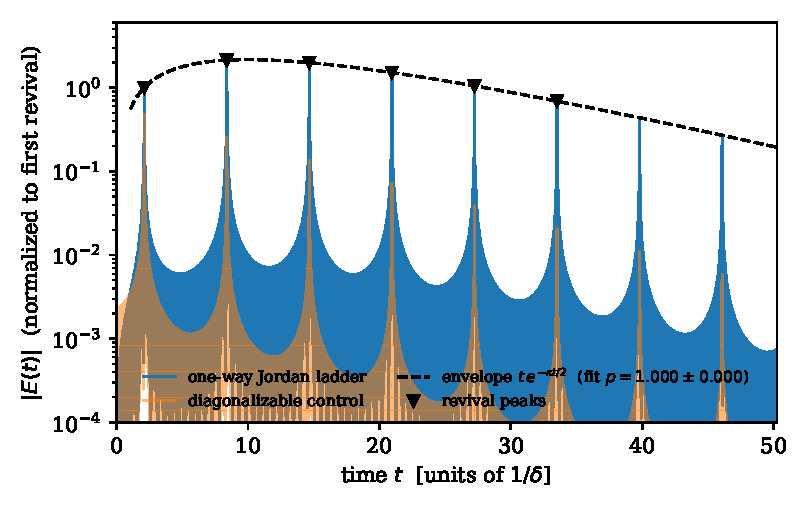
\includegraphics[width=0.82\textwidth]{figures/fig1_secular_envelope.pdf}
\caption{Simulation of the model of Section~\ref{sec:structure} in the mapped
dimensionless regime ($\kappa/\delta = 0.2$, $M = 300$ rungs, loop phase
$\phi = 2.1$): revival comb $|E(t)|$ of the one-way Jordan ladder versus the
diagonalizable control, with the secular envelope $t\,e^{-\kappa t/2}$
anchored on the fitted revival peaks. The three-regressor fit of
Section~\ref{sec:protocol} recovers $p = 1.0001 \pm 0.0001$ (Jordan
prediction $p=1$) and $\hat\kappa = 0.2000$. Deterministic model output; no
experimental data.}
\label{fig:envelope}
\end{figure}

\begin{figure}[t]
\centering
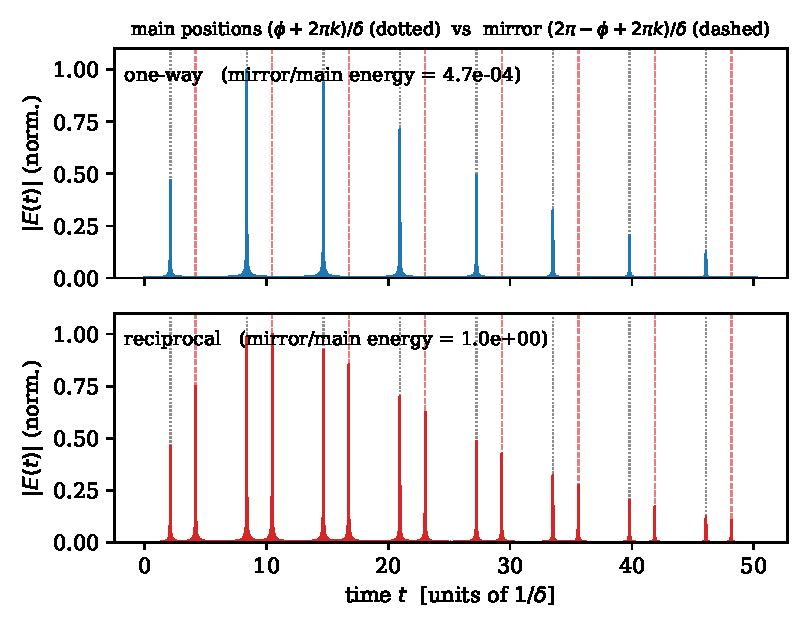
\includegraphics[width=0.82\textwidth]{figures/fig2_mirror_deletion.pdf}
\caption{The mirror-deletion law in the time domain (same model and
parameters as Fig.~\ref{fig:envelope}). Top: one-way configuration --- a
single revival comb at the main positions $(\phi + 2\pi k)/\delta$ (dotted);
the energy at the mirrored positions $(2\pi - \phi + 2\pi k)/\delta$ (dashed)
is at the numerical floor (mirror-to-main energy ratio $4.7\times 10^{-4}$).
Bottom: reciprocal control --- the twin comb appears at the mirrored
positions with ratio $\approx 1$. Deterministic model output; no experimental
data.}
\label{fig:mirror}
\end{figure}

\section{Noise and imperfection analysis}
\label{sec:noise}

\subsection{Classification and grouped channels}

For this protocol the decisive distinction is between within-record effects
(acting inside one 0.8-microsecond record, hence able to distort the secular
exponent) and between-shot effects (acting between averaged records, hence
damping the revival comb: a shot-to-shot loop-phase spread $\sigma$ suppresses
rung $m$ by $e^{-m^2 \sigma^2 / 2}$). Grouping ten physical effects by this
criterion and by channel yields four families: (A) loop phase noise (thermal,
acoustic, vibrational --- the fiber thermo-optic response is of order $10^3$
radians per kelvin over 20~m, so unstabilized drifts translate into radians
over an averaging run); (B) intensity noise (amplifier relative intensity noise
within the record; slow gain drift between shots); (C) polarization
(state-of-polarization drift converting, through polarization-dependent loss,
into slow amplitude fading); (D) parasitic reflections and finite isolation (a
genuine weak twin comb at the isolation floor; distributed Rayleigh backscatter
sits well below it for a 20~m loop). Kerr nonlinearity and third-order
dispersion are included as switches and shown negligible at milliwatt powers
(of order $10^{-5}$ radian per round trip, and $10^{-3}$ of the second-order
dispersion, respectively). All magnitudes are literature-typical and flagged as
such.

\subsection{Simulation results}

With additive detection noise alone, the secular exponent separates from the
diagonalizable value at the ten-sigma level in a single shot at amplitude
signal-to-noise 10, and at about forty sigma at signal-to-noise 3 with one
hundred oscilloscope averages. Replacing white noise by amplifier noise
recirculating on the loop resonances --- the least favorable spectral shape,
since the noise then peaks exactly where the signal lives --- degrades this
only mildly. The exponent is likewise unaffected by detector-bandwidth
truncation down to about fifteen rungs, by slow polarization fading, by gain
jitter, and, notably, by shot-to-shot loop-phase jitter: the secular envelope
of the revival peaks does not depend on the ladder size, so the Jordan
certificate survives phase noise that visibly destroys the comb. What phase
noise does destroy is the many-rung content of the comb --- the part of the
signal that carries the transcendental class --- with an effective ladder
$m_{\mathrm{eff}}$ of order $1/\sigma$. Loop dispersion is subcritical at the
mapped design and produces a clear failure signature (late revivals broadening
with revival index) only when exaggerated far beyond it. Finite laser linewidth
acts, after ensemble averaging, as an additional decay rate $\pi$ times the
linewidth: it biases the extracted $\kappa$ but provably not the exponent,
whose regressor is separated in the fit. Finally, two facts matter for the
conditional reciprocity witness: the isolation floor of a standard 40~dB
isolator lies below the realistic noise-floor of the twin-comb contrast, so
single-stage isolation suffices initially; and loop phase noise pollutes the
twin-comb contrast roughly tenfold before it kills the comb, so the witness
demands a phase-quiet loop even more than the comb itself does.

\subsection{Scope and ranking}

Within the explored window of literature-typical and stressed values, loop
phase stability dominates every other imperfection; intensity, polarization and
reflection channels are benign. We state the ranking with its exact scope: the
damage mechanisms and their scalings in the mode index are established in the
model; the ordering for a specific real device depends on the relative
magnitudes of its actual imperfections and remains to be established from
measured component data. The corresponding design guidance --- protect the loop
phase first --- is conditional on that window.

\section{Discussion and limitations}
\label{sec:discussion}

The additions of this version call for their own perimeter statement.
Sections~\ref{sec:boundary}--\ref{sec:spectroscopy} are structural
characterizations of the kernel as a mathematical object: machine-verified
simulation throughout, one elementary hand proof whose ingredients are
classical and labelled as such, and closed forms faced against the
simulations to their last digits. None of it adds a physical claim. The
log-periodic form is classical in the discrete-scale-invariance literature
(Section~\ref{sec:dsi}); what we read as potentially new --- the
hierarchy-free one-way route to it, and the jump-phase witness --- is
stated with the hedge it deserves, and its arbitration belongs to external
review, not to this deposit.

\subsection{Modeling assumptions}

Four idealizations deserve explicit statement. The mode families are taken as
ideal counter-winding ladders with a strictly linear frequency ladder; real
devices have dispersion, which we treat perturbatively in
Section~\ref{sec:noise} but which deforms the exact closed form. The one-way
coupling is Lindbladian and exact (the reverse element vanishes identically); a
physical isolator has finite isolation, which converts the exact statement
``the mirror partner is deleted'' into the quantitative statement ``the mirror
partner is suppressed to the isolation floor''. The laser is treated at the
ensemble level, where its finite linewidth becomes a deterministic additional
decay; individual records carry phase-diffusion realizations that the ensemble
treatment averages. Finally, every numerical value in
Sections~\ref{sec:platform}--\ref{sec:noise} is literature- or
catalogue-typical; none is a measurement of an actual component.

\subsection{What a measurement would and would not establish}

Observation of the three signatures --- secular exponent, phase-swept revival
comb, single-versus-twin comb down to the isolation floor --- would establish
the Jordan structure, the anti-holomorphic sector structure of the surviving
element (Section~\ref{sec:structure}), and the model-level comb suppression;
establishing strict unidirectionality $G_{12} = 0$ additionally requires the
reverse-injection configuration of Section~\ref{sec:protocol}. It would not
establish anything beyond that. In
particular it would carry no implication for arithmetic questions
(Section~\ref{sec:mock}), no statement about systems other than the one
measured, and no foundational or cosmological consequence. Conversely, the
measurement is informative in failure: each signature refutes a specific
structural claim, as follows.

\subsection{Falsifiability}

The proposal is refutable in parts. (i) If the secular envelope shows an
exponent consistent with zero under conditions where per-pair degeneracy and
one-way coupling are independently verified, the Jordan-ladder structure is
refuted. (ii) If the conversion channel of the two-point response depends on
the coordinate difference rather than the coordinate sum, the one-way kernel
structure is refuted. (iii) If a twin comb appears in the one-way configuration
at a contrast far above the independently measured isolation floor, the
mirror-deletion statement is refuted. (iv) The converse direction is bounded:
none of the three signatures, if observed, establishes more than the kernel
structure itself.

\subsection{Open questions}

Three questions are open at the level of mathematics. First, the exact status
of the resemblance to mock-modular completions: whether any map exists under
which the exchange operation realizes a modular transformation and the one-way
kernel arises as the shadow of a specific mock object; we possess no such map
and no argument excluding one. Second, the completeness of the classification:
our three formula-level properties separate all cases we have constructed, but
we have no theorem that they separate all kernels of physical origin. Third,
the boundary behavior: the closed form lives on the open unit polydisk and the
proposed measurement reads its boundary values; a rigorous treatment of the
boundary limit, in the presence of the complex ladder offset, would strengthen
Section~\ref{sec:platform}. A structural characterization of this boundary --- its intrinsic, dimensionless location, its emergence under truncation of the mode ladder, and the analytic continuation and branch structure beyond it --- is given in Section~\ref{sec:boundary}; the oriented (chiral) crossing law and the detuning-governed interference relief along the cut are characterized there as well; the rigorous limit statement remains open.

\section{Conclusion}

We have posed the removability question for anti-holomorphic structure in the
setting where, we argue, it is best posed --- the two-point transfer kernel of
a non-reciprocal open system --- and answered it at the level of certified
formula structure: one-way coupling between counter-winding mode ladders
produces a Lerch-transcendent kernel whose exchange-Hermitian mirror partner
is absent and whose reciprocity invariant $R = K - S(K)$, evaluated on the
complete two-point transfer kernel (the scalar closed form alone is
exchange-symmetric and blind to it), is non-zero --- two independent
violations that are both exhibited by the one-way construction at formula
level (they follow from $G_{12} = 0$ with nonvanishing transfer; they do not
by themselves characterize strict unidirectionality).
We have proposed a fiber-loop measurement of this structure, with an analysis
of its realistic imperfections and explicit criteria under which the proposal
would be refuted. No experimental data exist; the next step is a measurement.

\section*{Code and data availability}

The symbolic certification harness, the simulation scripts, and the findings
files underlying every certified claim in this paper are archived alongside
this deposit. This work extends the author's eml$^\star$ program on the
detection of anti-holomorphic dynamics; the corresponding paper and software
are archived at Zenodo under DOIs \href{https://doi.org/10.5281/zenodo.20272784}{10.5281/zenodo.20272784}
(paper) and \href{https://doi.org/10.5281/zenodo.20273262}{10.5281/zenodo.20273262}
(software), to which the present deposit is linked.

\section*{AI assistance disclosure}

The author, an independent researcher, developed this work with AI assistants
used as coding, auditing, and drafting tools under a strict verification
discipline: every symbolic claim was certified by exact Wirtinger-derivative
computation executed on the author's machine, and no numerical result reported
here was produced or accepted without such execution. Responsibility for the
content rests with the author.

\begin{thebibliography}{99}

\bibitem{Langbein2018}
W. Langbein,
\emph{No exceptional precision of exceptional-point sensors},
Phys. Rev. A \textbf{98}, 023805 (2018).

\bibitem{Wiersig2020}
J. Wiersig,
\emph{Review of exceptional point-based sensors},
Photonics Res. \textbf{8}, 1457--1467 (2020).

\bibitem{LauClerk2018}
H.-K. Lau and A. A. Clerk,
\emph{Fundamental limits and non-reciprocal approaches in non-Hermitian quantum sensing},
Nat. Commun. \textbf{9}, 4320 (2018).

\bibitem{Gardiner1993}
C. W. Gardiner,
\emph{Driving a quantum system with the output field from another driven quantum system},
Phys. Rev. Lett. \textbf{70}, 2269--2272 (1993).

\bibitem{Carmichael1993}
H. J. Carmichael,
\emph{Quantum trajectory theory for cascaded open systems},
Phys. Rev. Lett. \textbf{70}, 2273--2276 (1993).

\bibitem{MetelmannClerk2015}
A. Metelmann and A. A. Clerk,
\emph{Nonreciprocal photon transmission and amplification via reservoir engineering},
Phys. Rev. X \textbf{5}, 021025 (2015); arXiv:1502.07274.

\bibitem{Zwegers2002}
S. P. Zwegers,
\emph{Mock Theta Functions},
PhD thesis, Utrecht University (2002); arXiv:0807.4834.

\bibitem{Zagier2009}
D. Zagier,
\emph{Ramanujan's mock theta functions and their applications (after Zwegers and Ono--Bringmann)},
S\'eminaire Bourbaki, Exp. No. 986, Ast\'erisque \textbf{326} (2009).

\bibitem{DMZ2012}
A. Dabholkar, S. Murthy, and D. Zagier,
\emph{Quantum black holes, wall crossing, and mock modular forms},
arXiv:1208.4074.

\bibitem{DoraMoca2022}
B. D\'ora and C. P. Moca,
\emph{Full counting statistics in the many-body Hatano--Nelson model},
Phys. Rev. B \textbf{106}, 235125 (2022); arXiv:2208.12017.

\bibitem{DoraMoca2023}
B. D\'ora and C. P. Moca,
\emph{Work statistics and generalized Loschmidt echo for the Hatano--Nelson model},
arXiv:2310.19310 (2023).

\bibitem{Heiss2012}
W. D. Heiss,
\emph{The physics of exceptional points},
J. Phys. A: Math. Theor. \textbf{45}, 444016 (2012).

\bibitem{Dietz2007}
B. Dietz, T. Friedrich, J. Metz, M. Miski-Oglu, A. Richter, F. Sch\"afer,
and C. A. Stafford,
\emph{Rabi oscillations at exceptional points in microwave billiards},
Phys. Rev. E \textbf{75}, 027201 (2007).

\bibitem{BCOV1994}
M. Bershadsky, S. Cecotti, H. Ooguri, and C. Vafa,
\emph{Kodaira--Spencer theory of gravity and exact results for quantum string amplitudes},
Commun. Math. Phys. \textbf{165}, 311 (1994).

\bibitem{CecottiVafa1991}
S. Cecotti and C. Vafa,
\emph{Topological anti-topological fusion},
Nucl. Phys. B \textbf{367}, 359 (1991).

\bibitem{Vasilevski2000}
N. L. Vasilevski,
\emph{Poly-Fock spaces},
Oper. Theory Adv. Appl. \textbf{117}, 371--386 (Birkh\"auser, Basel, 2000).

\bibitem{Abreu2010}
L. D. Abreu,
\emph{Sampling and interpolation in Bargmann--Fock spaces of polyanalytic functions},
Appl. Comput. Harmon. Anal. \textbf{29}, 287--302 (2010).

\bibitem{AbreuFeichtinger2014}
L. D. Abreu and H. G. Feichtinger,
\emph{Function spaces of polyanalytic functions},
in \emph{Harmonic and Complex Analysis and its Applications}, Trends in Mathematics,
pp. 1--38 (Birkh\"auser, Cham, 2014).

\bibitem{McDonald2018} A.~McDonald, T.~Pereg-Barnea, and A.~A. Clerk, Phase-dependent chiral transport and effective non-Hermitian dynamics in a bosonic Kitaev-Majorana chain, Phys. Rev. X \textbf{8}, 041031 (2018).
\bibitem{LeeYang1952} C.~N. Yang and T.~D. Lee, Statistical theory of equations of state and phase transitions. I. Theory of condensation, Phys. Rev. \textbf{87}, 404 (1952); T.~D. Lee and C.~N. Yang, II. Lattice gas and Ising model, Phys. Rev. \textbf{87}, 410 (1952).
\bibitem{Nickel1999} B.~Nickel, On the singularity structure of the 2D Ising model susceptibility, J. Phys. A: Math. Gen. \textbf{32}, 3889 (1999); addendum, J. Phys. A: Math. Gen. \textbf{33}, 1693 (2000).
\bibitem{Caloz2018} C.~Caloz, A.~Al\`u, S.~Tretyakov, D.~Sounas, K.~Achouri,
and Z.-L. Deck-L\'eger, Electromagnetic nonreciprocity,
Phys. Rev. Applied \textbf{10}, 047001 (2018).
\bibitem{Silveirinha2019} M.~G.~Silveirinha, Hidden time-reversal symmetry in
dissipative reciprocal systems, Opt. Express \textbf{27}, 14328--14337 (2019).
\bibitem{Colom2023} R.~Colom et al., Crossing of the branch cut: the topological origin of a universal $2\pi$-phase retardation in non-Hermitian metasurfaces, Laser Photonics Rev. \textbf{17}, 2200976 (2023).
\bibitem{HuWang2023} Y.-M. Hu and Z.~Wang, Green's functions of multiband non-Hermitian systems, Phys. Rev. Research \textbf{5}, 043073 (2023).
\bibitem{Derrida1984} B.~Derrida, C.~Itzykson, and J.~M.~Luck,
Oscillatory critical amplitudes in hierarchical models,
Commun. Math. Phys. \textbf{94}, 115--132 (1984).

\bibitem{Sornette1998} D.~Sornette, Discrete-scale invariance and
complex dimensions, Phys. Rep. \textbf{297}, 239--270 (1998).

\bibitem{Bohr1947} H.~Bohr, \emph{Almost Periodic Functions}
(Chelsea, New York, 1947).

\bibitem{Wanjura2020} C.~C.~Wanjura, M.~Brunelli, and A.~Nunnenkamp,
Topological framework for directional amplification in driven-dissipative
cavity arrays, Nat. Commun. \textbf{11}, 3149 (2020).

\bibitem{Zirnstein2021} H.-G.~Zirnstein, G.~Refael, and B.~Rosenow,
Bulk-boundary correspondence for non-Hermitian Hamiltonians via Green
functions, Phys. Rev. Lett. \textbf{126}, 216407 (2021).

\end{thebibliography}

\end{document}
